\newpage 

\section{Transactions and Concurrency Control}
\subsection{Optimistic Concurrency Control (OCC)}

\noindent
Say the backbone of our stock trading application is a 
distributed database. The system may conduct complicated
stock trades based on server stock prices.
\begin{figure}[h]
    \centering
    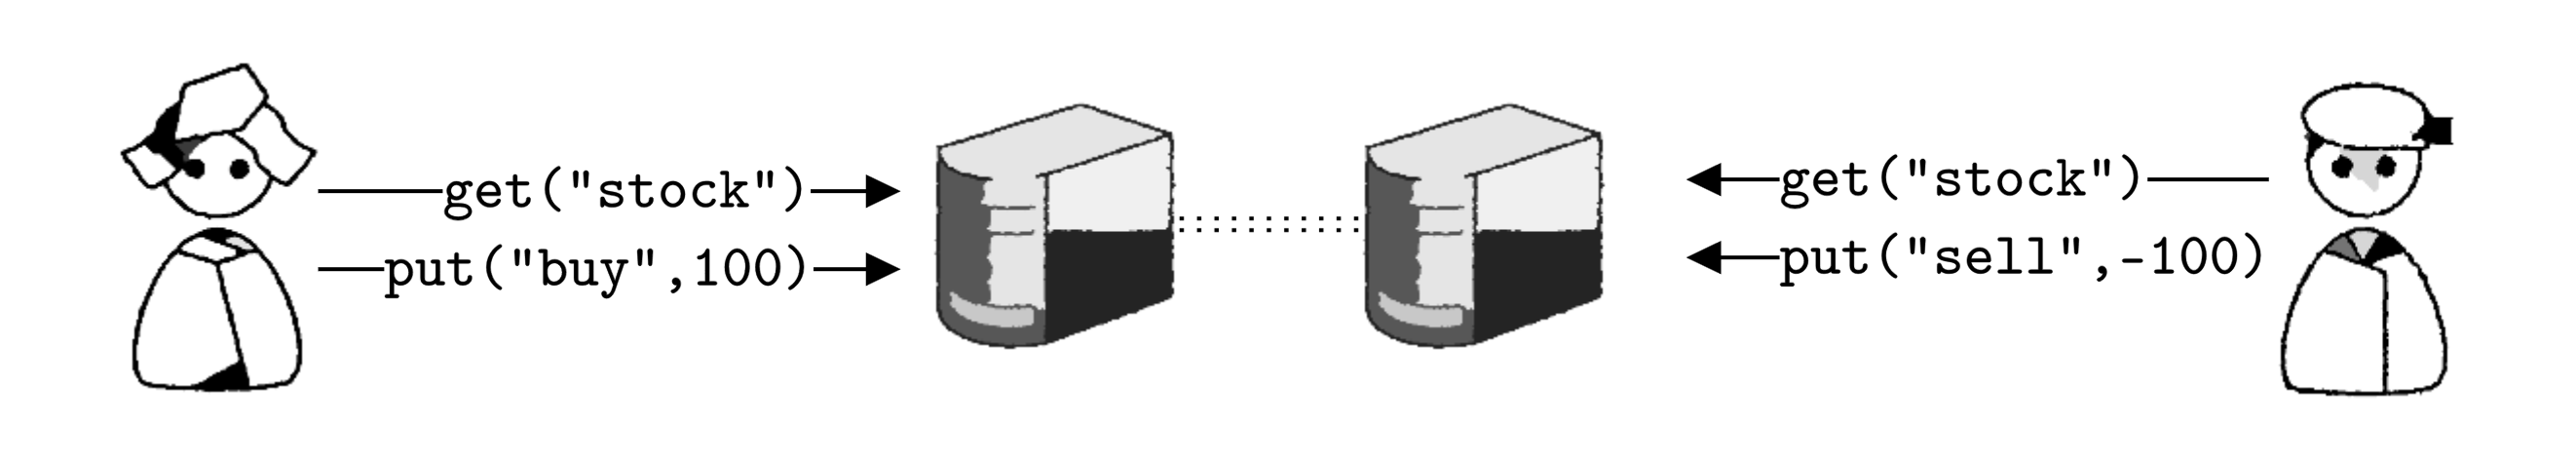
\includegraphics[width=\textwidth]{Sections/trans/stock.png}
    \caption{Two users checking the stock prices and making a trade based on such information.}
    \label{fig:stock_trading}
\end{figure}

\noindent
It is critical that the stock price is consistent through all servers, and 
more important that if any trade fails, the system can recover to a consistent state.

\begin{Def}[Transaction]

    A \textbf{transaction} is a sequence of operations that are treated as a single unit of work.
    A transaction must satisfy the \textbf{ACID} properties:
    \begin{itemize}
        \item \textbf{Atomicity}: A transaction is either fully completed or dropped entirely.
        \item \textbf{Consistency}: A transaction must leave the database in a consistent state.
        \item \textbf{Isolation}: Transactions must be isolated from each other.
        \item \textbf{Durability}: Once a transaction is committed, it remains so even after system failure.
    \end{itemize}
\end{Def}

\vspace{-0.5em}
\begin{figure}[h]
    \centering 
    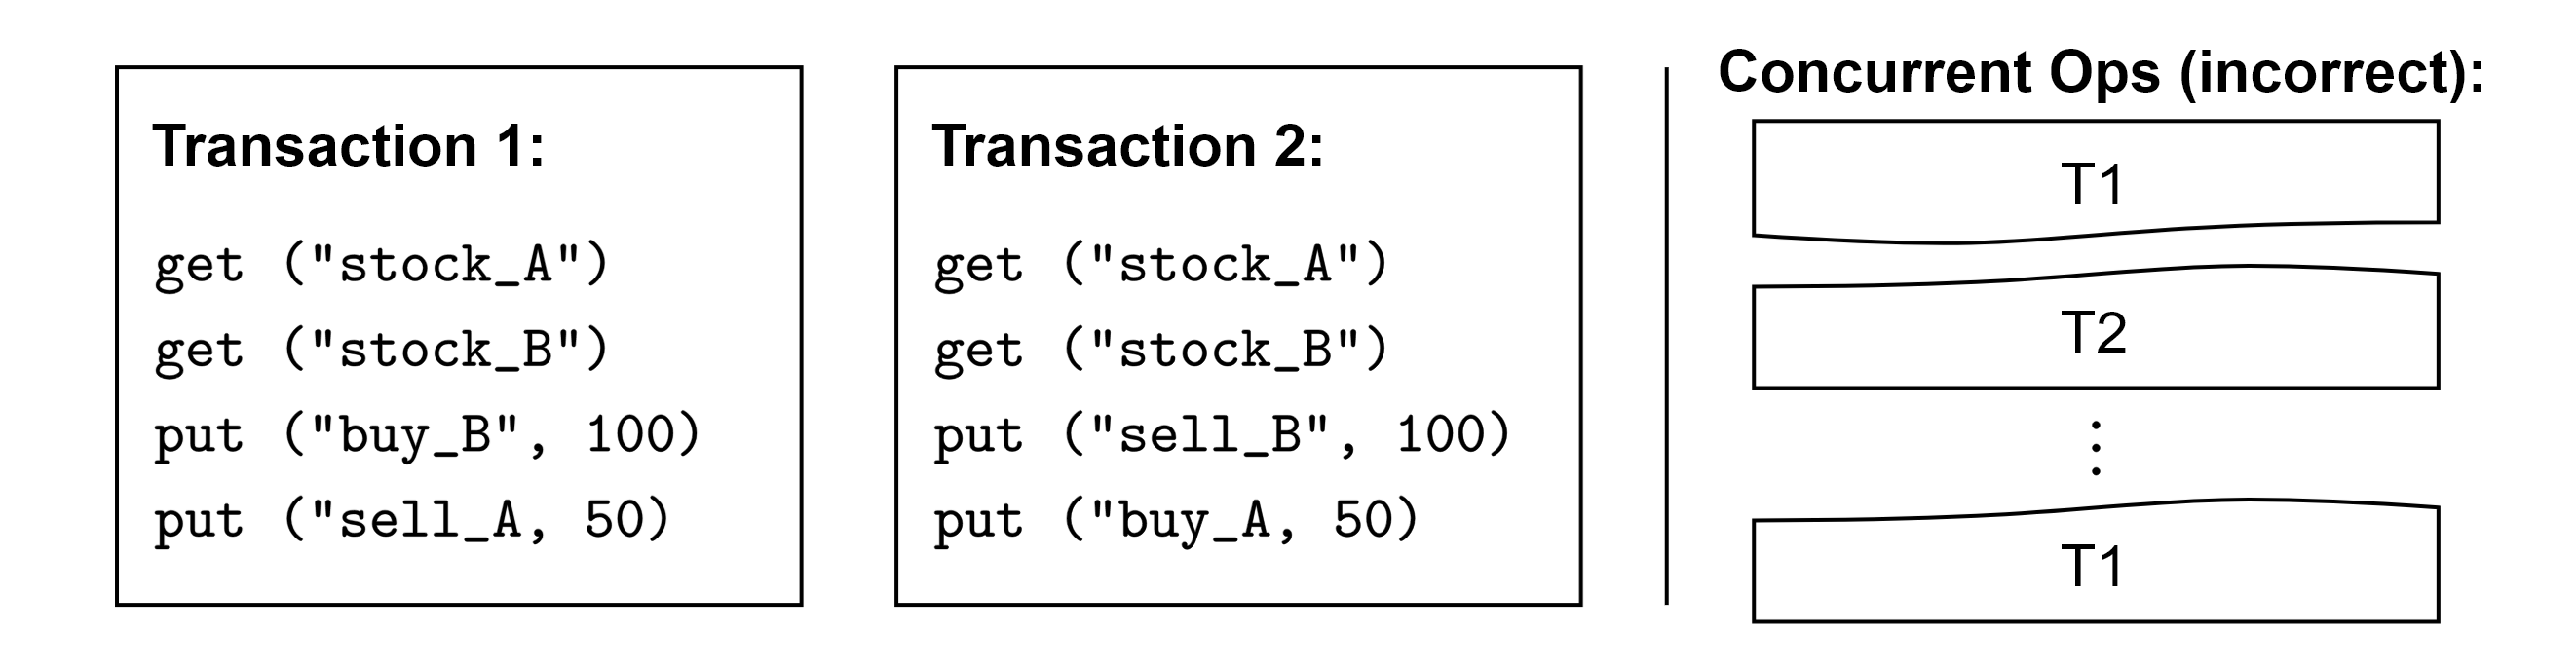
\includegraphics[width=\textwidth]{Sections/trans/stock_2.png}
    \caption{Two transactions which whose operations are interleaved.}
    \label{fig:stock_trading}
\end{figure}

\noindent
Interleaving transactions \textbf{violates the isolation property}. This is problematic in 
Figure (\ref{fig:stock_trading}) as T2's (transaction 2) operations may depend on the server 
state before T1's transaction. Additionally partially completed transactions leave the system in an inconsistent state, violating
\textbf{atomicity}
(e.g., T1's ``buy\_B'' fails, but ``sell\_A'' succeeds).

\newpage

\noindent
We discuss another consistency model which will help us in this settings:
\begin{Def}[Serializability]

    \label{def:serializability}
    
    \textbf{Serializability} is a strong consistency model that ensures the outcome of concurrent transactions is the same as if they were executed in some sequential (serial) order.\\
    
    \noindent
    This differs from \textbf{linearizability}, which focuses on the real-time ordering of individual operations. Serializability instead concerns the logical order of \textbf{entire transactions}, independent of their timing.\\ 

    \noindent
    However, \textbf{strict-serializability} does care about real-time ordering in addition to the logical order of transactions. This implies linearizability, but not vice versa.
    
    \end{Def}

\noindent
We consider the following model to help us preform transactions:
\begin{Def}[Optimistic Concurrency Control (OCC)]

    \textbf{Optimistic Concurrency Control (OCC)} assumes conflicts are rare and proceeds without locking. It follows four main steps:
    
    \begin{itemize}
        \item \textbf{Prepare}: The system reads the transaction request and creates a backup or temporary copy of the state.
        \item \textbf{Modify/Validate}: The transaction modifies the temporary state. Then The system checks whether the transaction is \textbf{serializable}.
        \item \textbf{Commit/Rollback}: If valid, commit; Otherwise, abort transaction and rollback to previous state.
    \end{itemize}
    
    \noindent
    \underline{This only solves \textbf{isolation},} as it does \textbf{not} guarantee atomicity.
    \end{Def}
    \begin{Def}[Transaction Coordinator and Database Servers]

        OCC maintains two necessary components: 
        
        \begin{itemize}
            \item \textbf{Transaction Coordinator (TC)}: The validation server responsible for checking whether a transaction is \textbf{serializable}. It receives requests from clients and responds with either:
            \begin{itemize}
                \item \texttt{OK}: if the transaction is serializable,
                \item \texttt{ABORT}: if it conflicts with prior transactions.
            \end{itemize}
        
            \item \textbf{Database Servers}: Receives transaction operations, executing it on local state. Then, on \textbf{OK}---commit state, on \textbf{ABORT}---rollback to the previous state.
        
        \end{itemize}        
        \end{Def}
        
    \newpage 

    \noindent
    We consider one model, which where multiple clients interact with one TC.
    \begin{Example}[Centralized OCC]

        Consider these two examples with a single TC and multiple clients on the network line:\\

       \noindent
        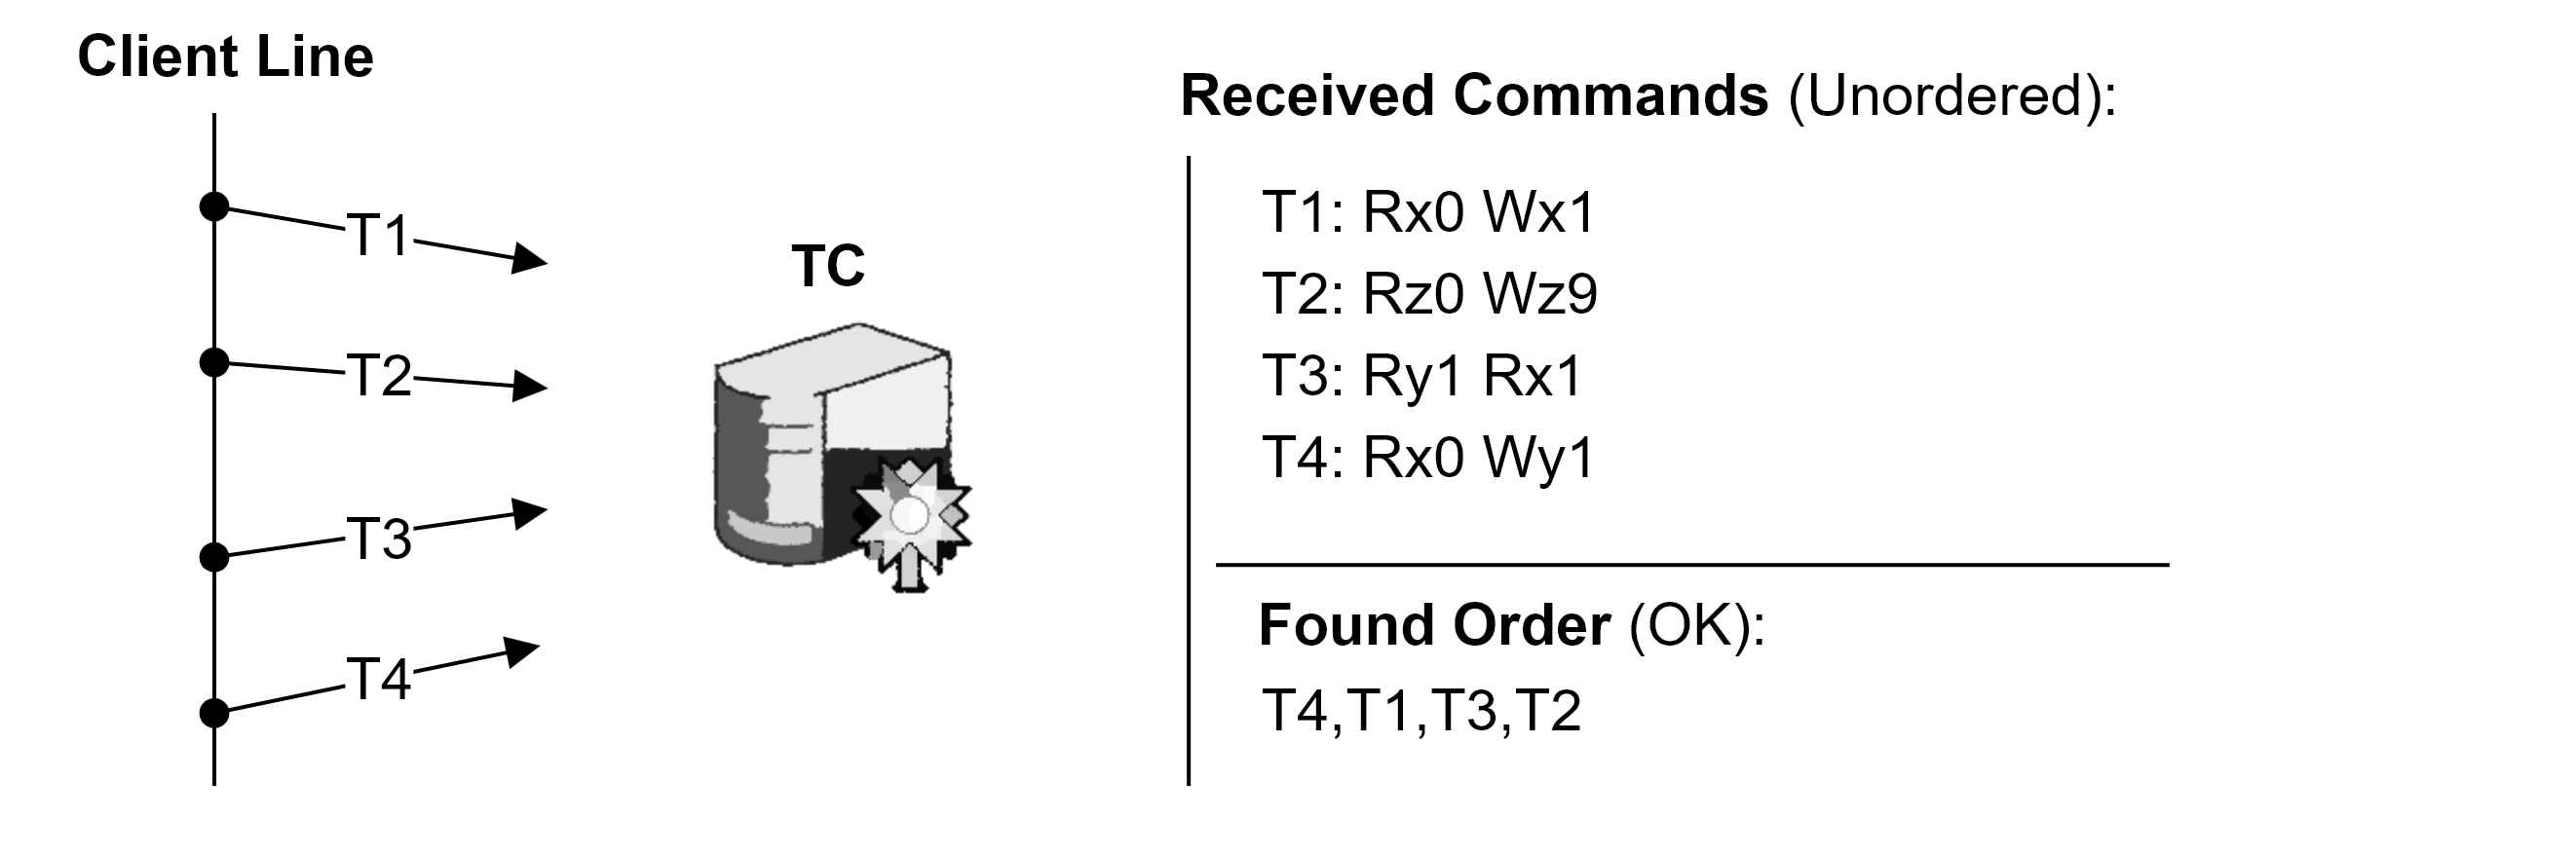
\includegraphics[width=\textwidth]{Sections/trans/central_1.png}
           
        \noindent
        Here, clients on the line send transactions T1--T4 to the TC. The TC then checks the transactions for serializability.
        In this case an order is found (T4,T1,T3,T2), which the TC communicates to the DBs to commit.\\

        \noindent
        \rule{\textwidth}{0.4pt}\\

        \noindent
        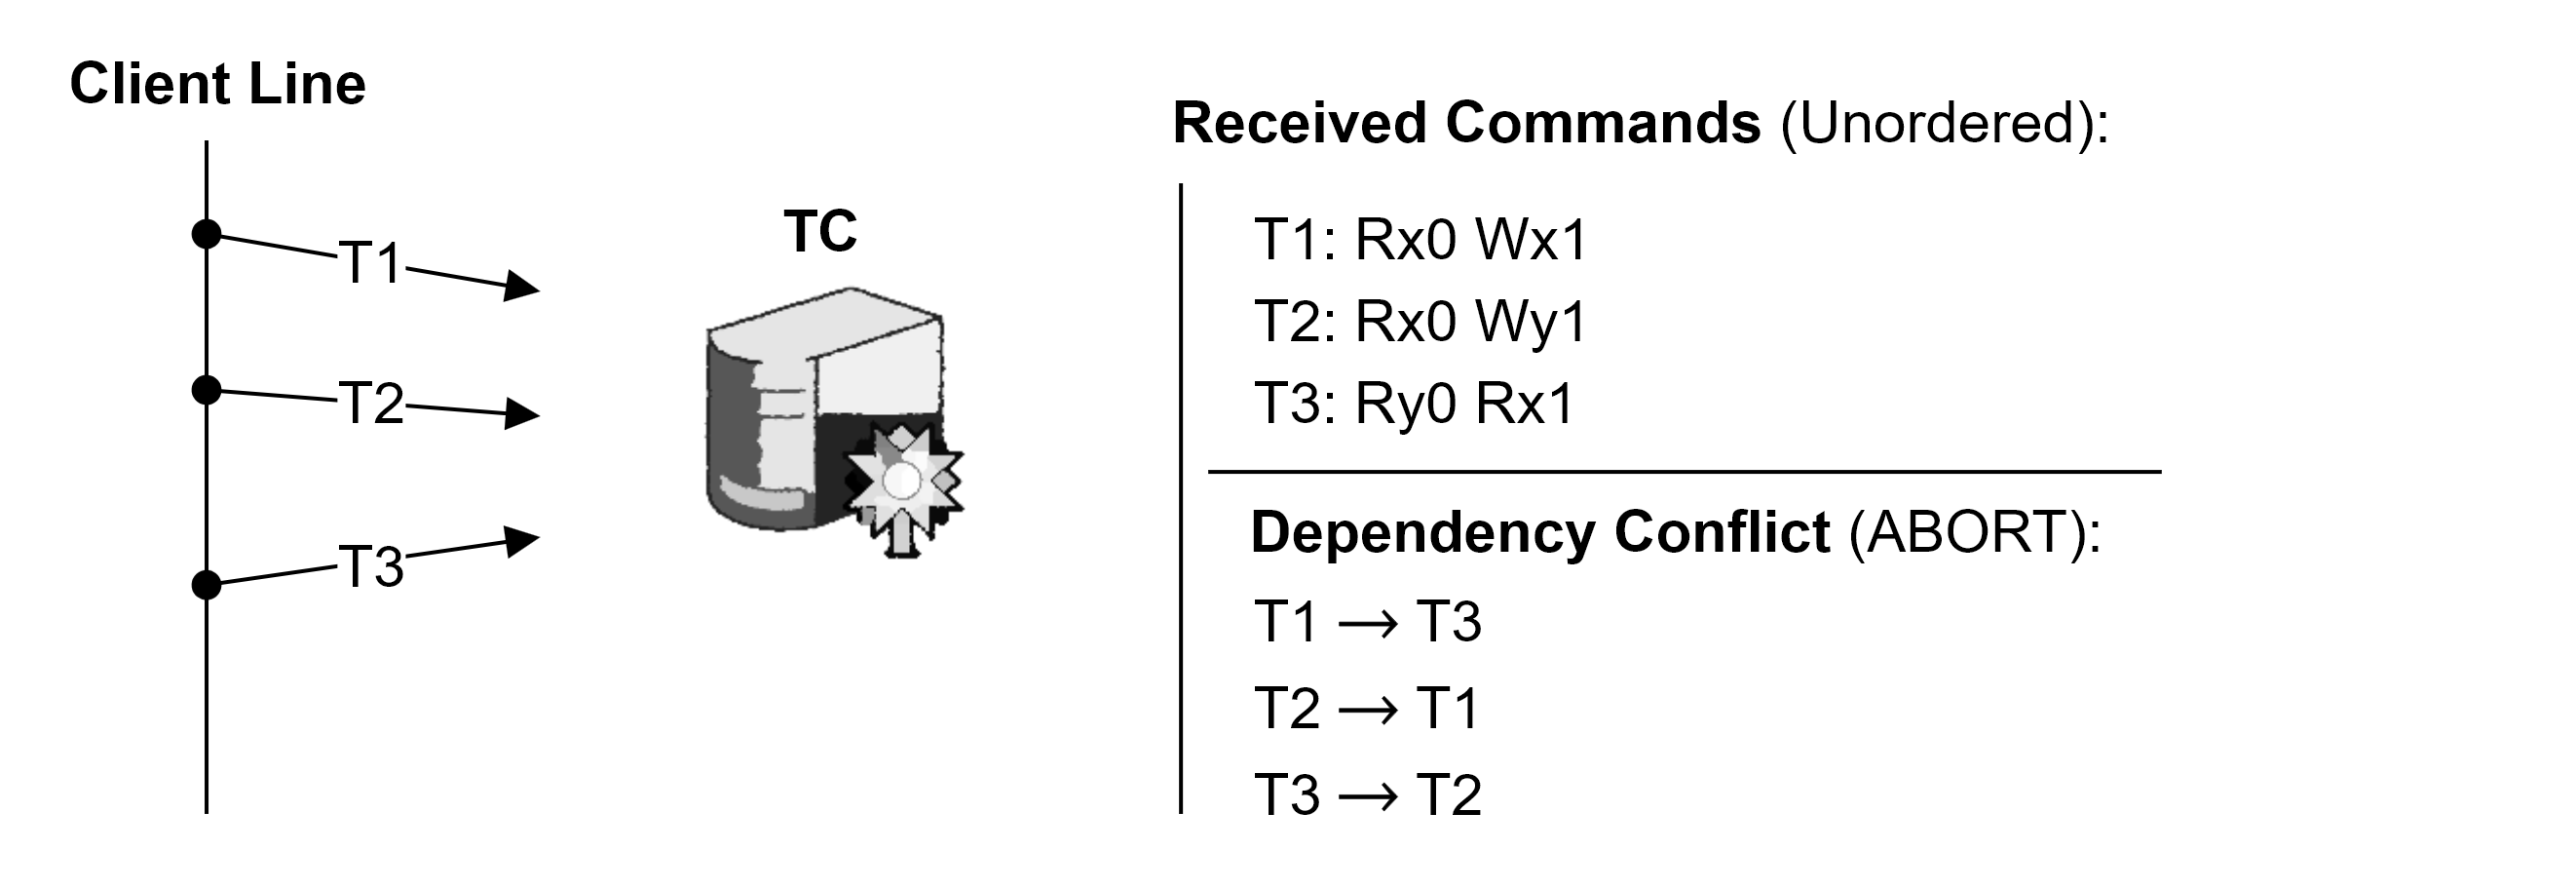
\includegraphics[width=\textwidth]{Sections/trans/central_2.png}

        \noindent
        Here, transaction requests, T1, T2, and T3, do not have a serial order.
        As we build, T1 $\to$ T3 (T1 then T3) makes logical sense. Then T2 $\to$ T3, giving us the order T2 $\to$ T1 $\to$ T3;
        However, it appears T3 must come before T2. This causes a cycle (T2 $\to$ T1 $\to$ T3 $\to$ T2).
        Hence, the TC must must abort all transactions.
    \end{Example}

    \begin{Tip}
    If familiar with \textbf{Directed Acyclic Graphs (DAG)}, one can think of the transactions as nodes and the edges as the dependencies between them.
    If the graph is a DAG, then there is some serial order (OK). If not, then there is a cycle, so we must abort.
    \end{Tip}

    \newpage

    \noindent
    Though we run into an issue when there are multiple TCs.
    \begin{Example}[Distributed OCC]

        Consider two TCs responsible for different parts of our system data.

        \noindent
        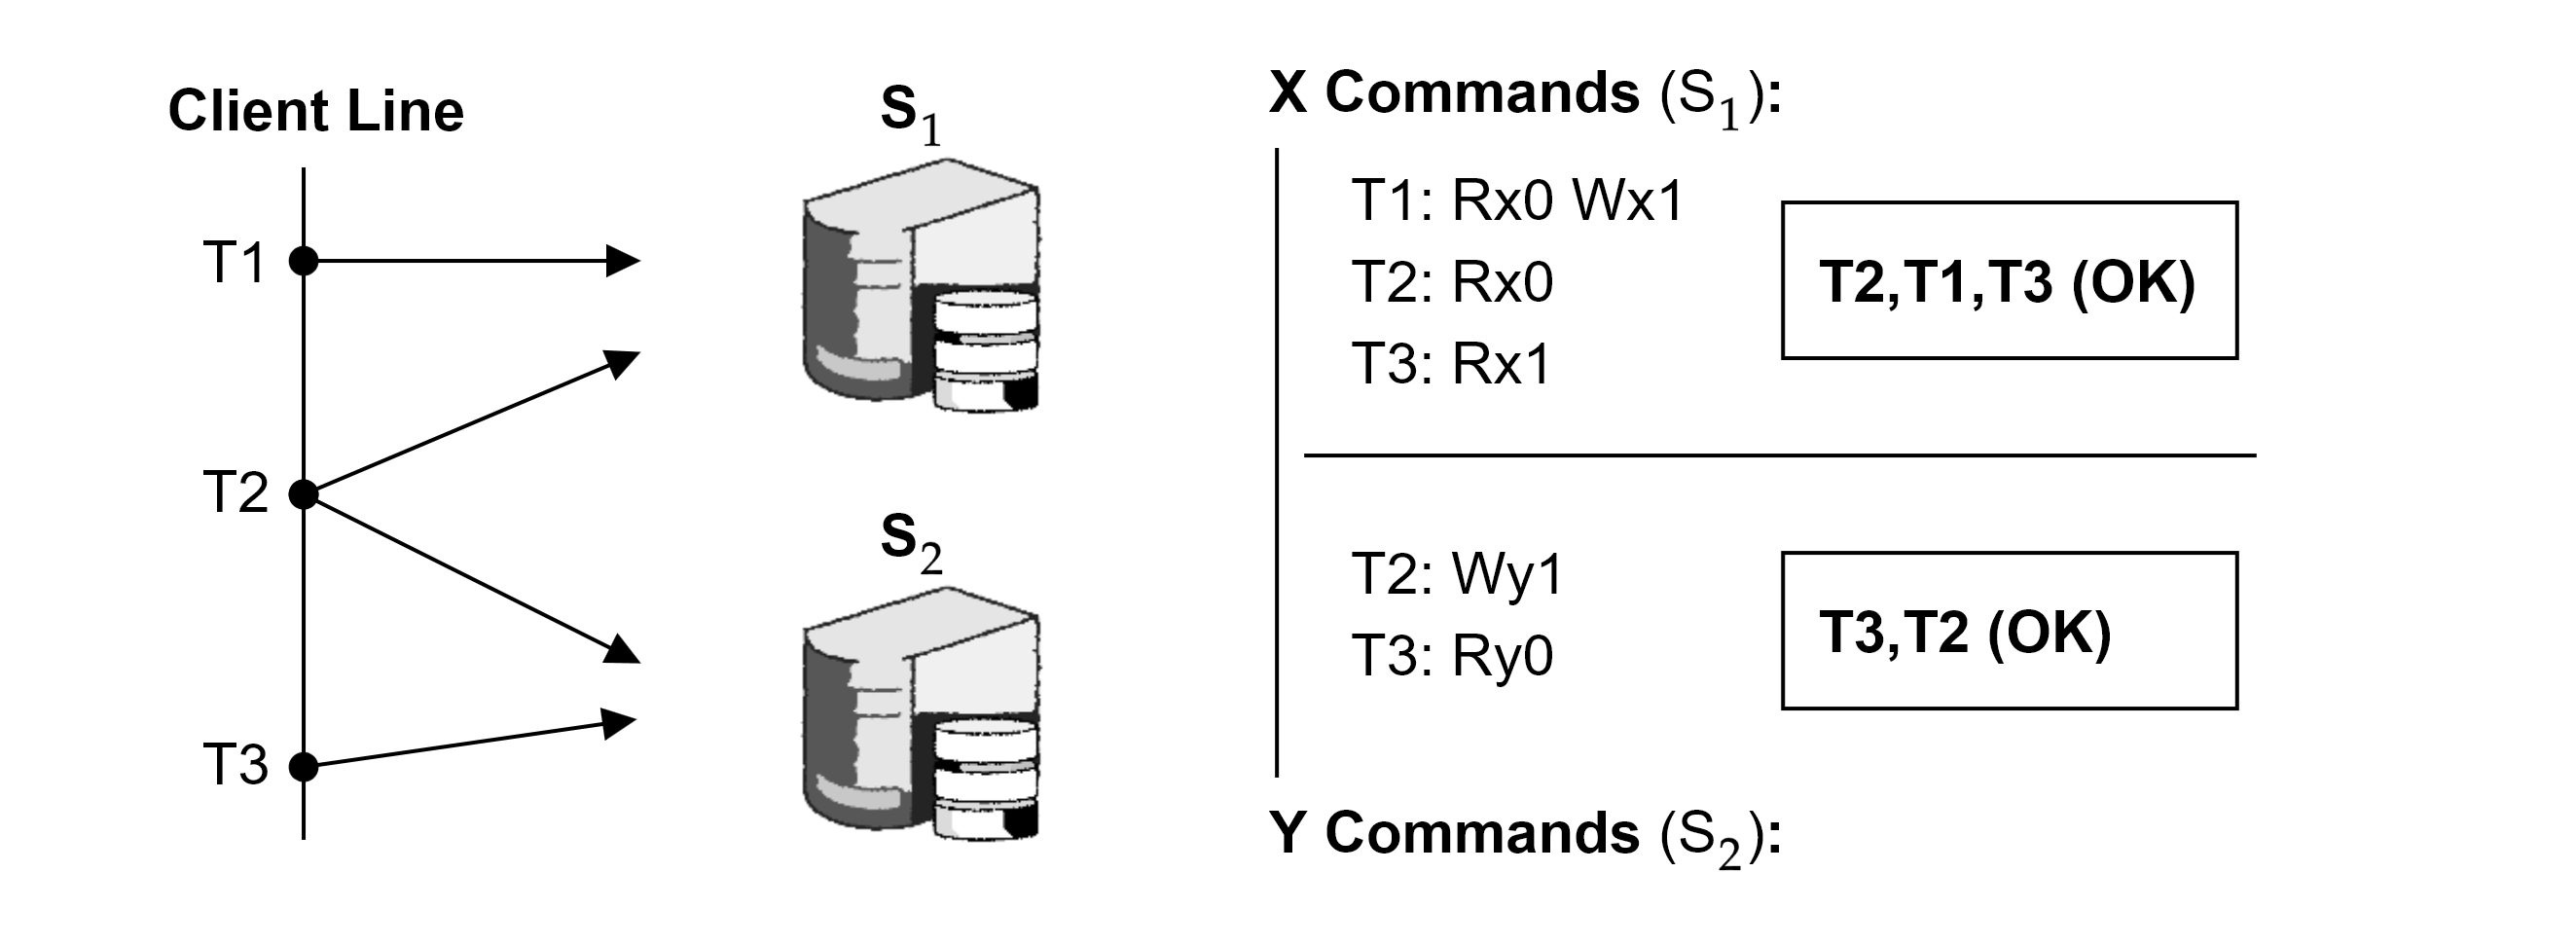
\includegraphics[width=\textwidth]{Sections/trans/central_3.png}

        \noindent
        The problem occurs as TC$_1$ and TC$_2$ pick \textbf{different serial orders} for the transactions.
    \end{Example}
    
\begin{theo}[Timestamping Distributed OCC]

    \textbf{Timestamping} is a method where each transaction is assigned a unique timestamp (ID), which aids
    order agreement between TCs.
\end{theo}

\begin{Example}[Timestamping Distributed OCC]

    \vspace{-1em}
    \noindent
    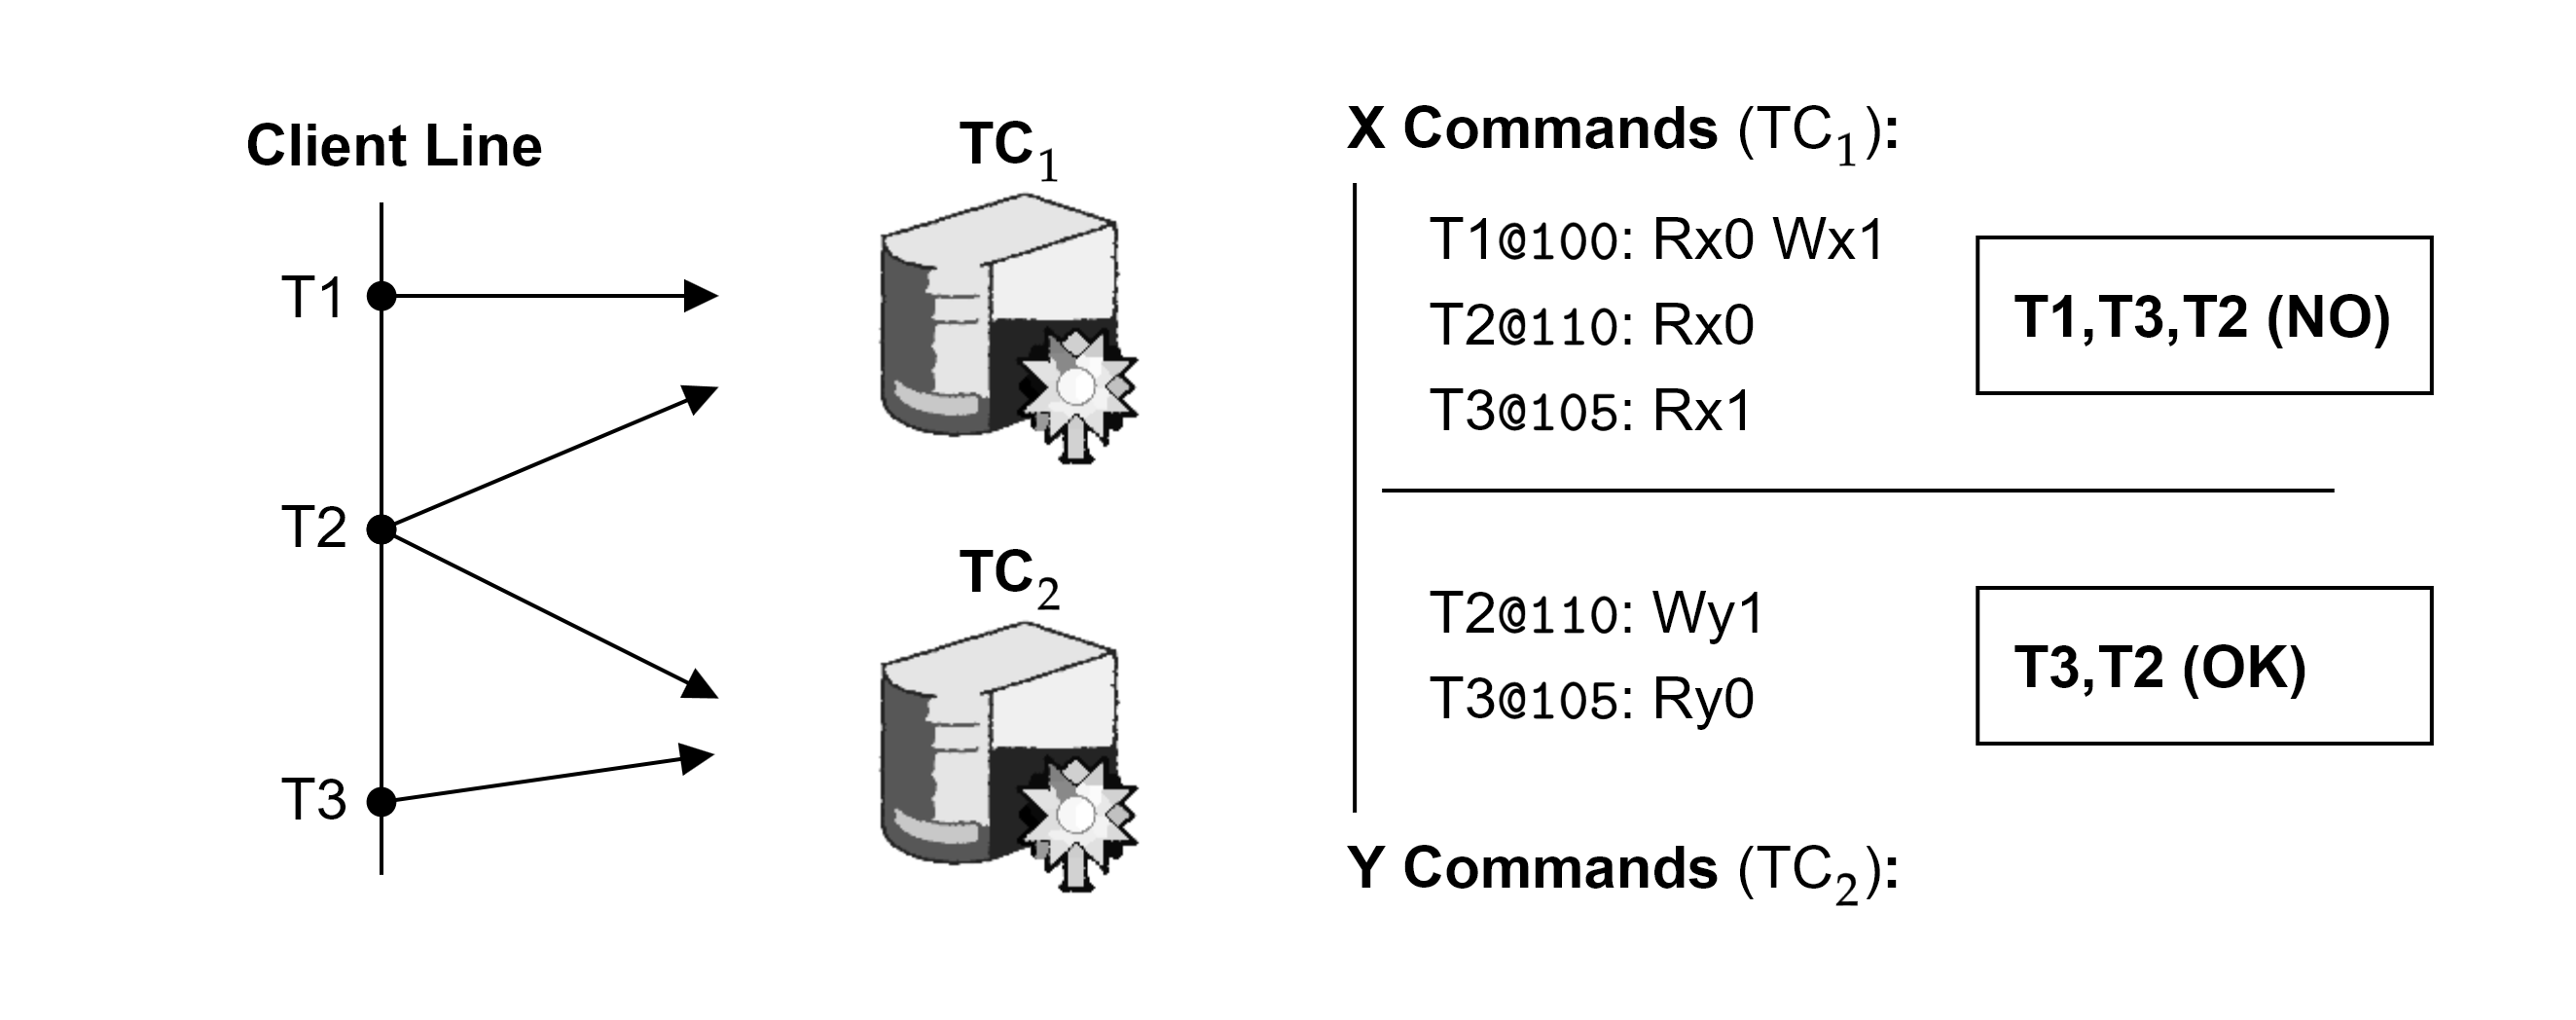
\includegraphics[width=\textwidth]{Sections/trans/central_4.png}

    \noindent
    \underline{\textbf{Timestamps (@\#) are only serve as IDs.}} Here TC$_2$ OKs the order (T3,T2). TC$_1$ sees this,
    enforces the order, but is not able to serialize (T1,T3,T2). Hence, it aborts (NO).
    \end{Example}

    \newpage 

\subsection{Two-Phase Commit (2PC)}
    
